\section{Classification}

To attempt classification, one method is to use linear regression and map all predictions greater than 0.5 as a 1 and all less than 0.5 as a 0. However, this method doesn't work well because classification is not actually a linear function.\\

The classification problem is just like the regression problem, except that the values we now want to predict take on only a small number of discrete values. For now, we will focus on the binary classification problem in which y can take on only two values, 0 and 1. (Most of what we say here will also generalize to the multiple-class case.) For instance, if we are trying to build a spam classifier for email, then $x^{(i)}$  may be some features of a piece of email, and y may be 1 if it is a piece of spam mail, and 0 otherwise. Hence, $y \in {0,1}$. 0 is also called the negative class, and 1 the positive class, and they are sometimes also denoted by the symbols “-” and “+.” Given $x^{(i)}$ the corresponding $y^{(i)}$ is also called the label for the training example.\\

Classification problems:\\
Email: Spam/Not Spam\\
Online Transaction: Valid/Fraud\\
Tumor: Malignant/Benign\\
$y \in {0,1}$ where 0 is the negative class and 1 is the positive class.\\

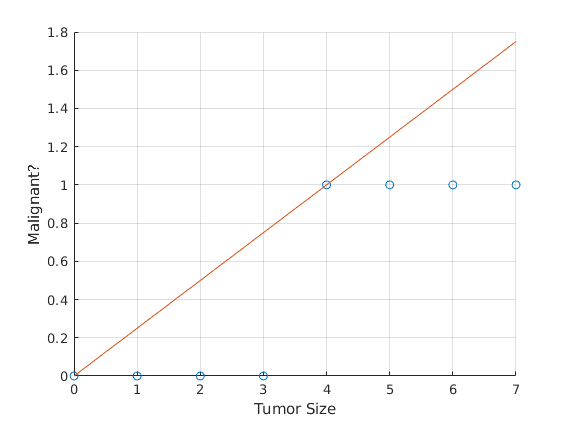
\includegraphics{matlab/classification.png}
For a few points that split up like this easily, the linear fit is not good.\\

Threshold Classifier output $h_{\theta}(x)$ at 0.5\\
if $h_{\theta}(x) \geq$ 0.5 y=1\\
if $h_{\theta}(x) <$ 0.5 y= 0\\
This is not perfect, still can mis-classify somethings.  It might be a reasonable solution. An outlier can skew the line.  This can move the thresold to the wrong location.  Linear regression is not a great idea for classification.

Logistic Regression outputs are always between 0 and 1.  The name includes regression but it is a classification algorithm\\
$$
0 \leq h_{\theta}(x) \leq 1
$$

\subsubsection{Hypothesis Representation}

We could approach the classification problem ignoring the fact that y is discrete-valued, and use our old linear regression algorithm to try to predict y given x. However, it is easy to construct examples where this method performs very poorly. Intuitively, it also doesn’t make sense for $h_\theta (x)$ to take values larger than 1 or smaller than 0 when we know that $y \in {0, 1}$. To fix this, let’s change the form for our hypotheses $h_\theta (x)$ satisfy $0 \leq h_\theta (x) \leq 1$. This is accomplished by plugging $\theta^Tx$ into the Logistic Function.


Our new form uses the "Sigmoid Function," also called the "Logistic Function":
\begin{equation}
  \begin{aligned}
    h_{\theta}(x) &= g(\theta^{T}x)\\
    z &= \theta^{T}x \\
    g(z) &= \frac{1}{1+e^{-z}}\\
    h_{\theta}(x) &= \frac{1}{1+e^{-\theta^{T}x}}
  \end{aligned}
\end{equation}

$g(z)$ is the Sigmoid or Logistic Function.  This is where the name Logistic Regression comes from.\\

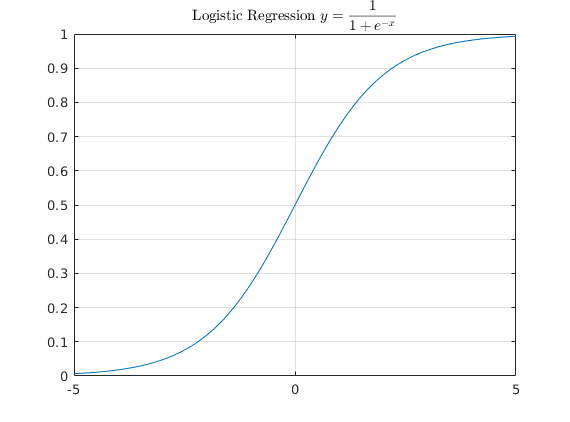
\includegraphics{matlab/logistic_plot.png}

The function g(z), shown here, maps any real number to the (0, 1) interval, making it useful for transforming an arbitrary-valued function into a function better suited for classification.\\


$h_{\theta}(x)$ will give us the probability that our output is 1. For example, $h_\theta(x)=0.7$ gives us a probability of 70\% that our output is 1. Our probability that our prediction is 0 is just the complement of our probability that it is 1 (e.g. if probability that it is 1 is 70\%, then the probability that it is 0 is 30\\

\begin{equation}
  \begin{aligned}
  &h_\theta(x) = P(y=1 \| x ; \theta) &= 1 - P(y=0 | x ; \theta) \\
  &P(y = 0 \| x;\theta) + P(y = 1 | x ; \theta) = 1
  \end{aligned}
\end{equation}

Fit parameters $\theta$ to our data.\\
$h_{\theta}(x)$ = estimate probability that y=1 on input x\\


Example:\\
$
x =
\begin{bmatrix}
  x_{0} \\
  x_{1} \\
\end{bmatrix}
$ =
$
\begin{bmatrix}
  1 \\
  tumor size \\
\end{bmatrix}
$\\

If $h_{\theta}(x)$ = 0.7, then it is a 70\% chance of being a tumor.


\subsubsection{Decision Boundary}

In order to get our discrete 0 or 1 classification, we can translate the output of the hypothesis function as follows:
\begin{equation}
  \begin{aligned}
    & h_\theta(x) \geq 0.5 \rightarrow y = 1 \\
    & h_\theta(x) < 0.5 \rightarrow y = 0 \\
  \end{aligned}
\end{equation}

The way our logistic function g behaves is that when its input is greater than or equal to zero, its output is greater than or equal to 0.5:

\begin{equation}
  \begin{aligned}& g(z) \geq 0.5 \\
    & when \; z \geq 0\end{aligned}
\end{equation}

Remember.

\begin{equation}
  \begin{aligned}
    z=0, e^{0}=1 \Rightarrow g(z)=1/2\\
    z \to \infty, e^{-\infty} \to 0 \Rightarrow g(z)=1\\
    z \to -\infty, e^{\infty}\to \infty \Rightarrow g(z)=0
  \end{aligned}
\end{equation}

So if our input to g is $\theta^{T}X$ then that means:
\begin{equation}
  \begin{aligned}
    & h_\theta(x) = g(\theta^T x) \geq 0.5 \\
    & when \; \theta^T x \geq 0
  \end{aligned}
\end{equation}

From these statements we can now say:
\begin{equation}
  \begin{aligned}
    & \theta^T x \geq 0 \Rightarrow y = 1\\
    & \theta^T x < 0 \Rightarrow y = 0 \\
  \end{aligned}
\end{equation}

The \textbf{decision boundary} is the line that separates the area where y = 0 and where y = 1. It is created by our hypothesis function.

Example:
\begin{equation}
  \begin{aligned}
    & \theta = \begin{bmatrix}
      5\\
      -1\\
      0\\
    \end{bmatrix}\\
     & y = 1 \; if \; 5 + (-1) x_1 + 0 x_2 \geq 0\\
     & 5 - x_1 \geq 0\\
     & - x_1 \geq -5\\
    & x_1 \leq 5\\
     \end{aligned}
\end{equation}

In this case, our decision boundary is a straight vertical line placed on the graph where $x_1$ =5, and everything to the left of that denotes y = 1, while everything to the right denotes y = 0.\\

Again, the input to the sigmoid function g(z) (e.g. $\theta^T X$ doesn't need to be linear, and could be a function that describes a circle (e.g. z = $\theta_0 + \theta_1 x_1^2 +\theta_2 x_2^2$ or any shape to fit our data.

Example:\\
If $h_{\theta}(x) = g(\theta_{0} + \theta_{1}x_{1} + \theta_{2}x_{2})$ then predict y =1.\\
For given $ \theta = \begin{bmatrix}
  -3\\
  1\\
  1\\
\end{bmatrix}$\\
then $ -3 + x_{1} + x_{2} \geq 0 $.\\
This means $\theta^{T}x = -3 + x_{1} + x_{2} + \theta_{3}x_{1}^{2} + \theta_{4}x_{2}^{2})$\\

\textbf{Non-Linear Decision Boundaries}
$h_{\theta}(x) = g(\theta_{0} + \theta_{1}x_{1} + \theta_{2}x_{2}$\\
$
\begin{aligned}
  & \theta = \begin{bmatrix}
    -1\\
    0\\
    0\\
    1\\
    1\\
  \end{bmatrix}
\end{aligned}\\
$\\
This will predict y =1 if $-1 + x_{1}^{2} + x_{2}^{2} \geq 0$

Decision Boundary is property not of training set but of the hypothesis and parameters. \\

You can use even higher order polynomials leading to very complex decision boundaries.

\subsection{Logistic Regression Model}
\subsubsection{Cost Function}

We cannot use the same cost function that we use for linear regression because the Logistic Function will cause the output to be wavy, causing many local optima. In other words, it will not be a convex function.\\

Instead, our cost function for logistic regression looks like:
\begin{equation}
  \begin{aligned}
    & J(\theta) = \dfrac{1}{m} \sum_{i=1}^m \mathrm{Cost}(h_\theta(x^{(i)}),y^{(i)}) \\
    & \mathrm{Cost}(h_\theta(x),y) = -\log(h_\theta(x)) \; & \text{if y = 1} \\
    & \mathrm{Cost}(h_\theta(x),y) = -\log(1-h_\theta(x)) \; & \text{if y = 0}
  \end{aligned}
\end{equation}

When y = 1, we get the following plot for $J(\theta) vs h_{\theta}(x)$\\
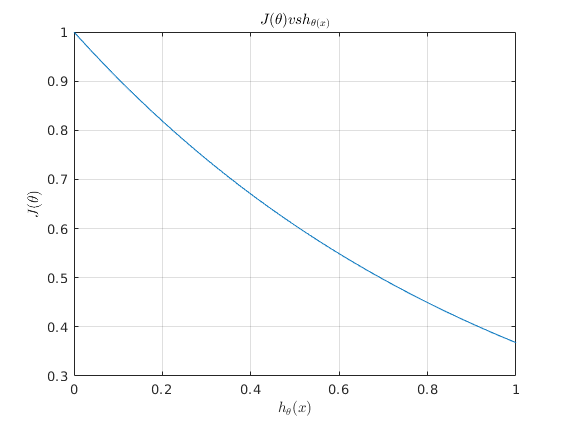
\includegraphics{matlab/logistic_cost_1.png} \\


When y = 0, we get the following plot for $J(\theta) vs h_{\theta}(x)$\\
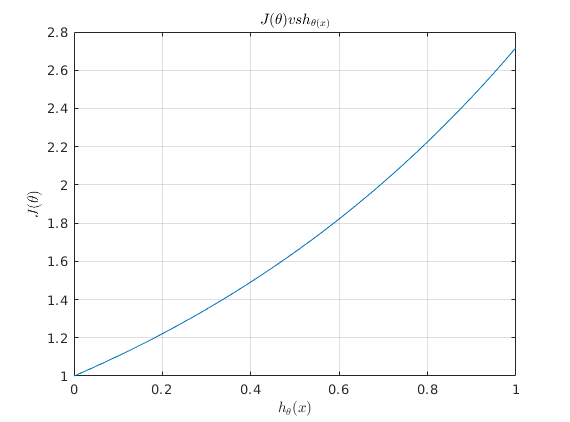
\includegraphics{matlab/logistic_cost_2.png} \\

\begin{equation}
  \begin{aligned}
    & \mathrm{Cost}(h_\theta(x),y) = 0 \text{ if } h_\theta(x) = y \newline
    & \mathrm{Cost}(h_\theta(x),y) \rightarrow \infty \text{ if } y = 0 \; \mathrm{and} \; h_\theta(x) \rightarrow 1 \newline
    & \mathrm{Cost}(h_\theta(x),y) \rightarrow \infty \text{ if } y = 1 \; \mathrm{and} \; h_\theta(x) \rightarrow 0 \newline
  \end{aligned}
\end{equation}

If our correct answer 'y' is 0, then the cost function will be 0 if our hypothesis function also outputs 0. If our hypothesis approaches 1, then the cost function will approach infinity.\\

If our correct answer 'y' is 1, then the cost function will be 0 if our hypothesis function outputs 1. If our hypothesis approaches 0, then the cost function will approach infinity.\\

Note that writing the cost function in this way guarantees that $J(\theta)$ is convex for logistic regression.\\ 


\textbf{Problem:}\\
How to choose parameters $\theta$?\\
Training Set: ${(x^{(1)}, y^{(1)}), (x^{(2)}, y^{(2)}), (x^{(3)}, y^{(3)}) ... (x^{(m)}, y^{(m)}) }$\\
m example $x \in   \begin{aligned}
  & \begin{bmatrix}
    x_{0}\\
    x_{1}\\
    \vdots\\
    x_{n}\\    
    \end{bmatrix}
\end{aligned}
  $\\

  With $x_{0}=1$ and $y \in {0,1}$ this mean y must be 0 or 1.\\
  $h_{\theta}(x) = \frac{1}{1+e^{\theta^{T}X}}$\\

  
  Linear Regression Cost:
  \begin{equation}
    J(\theta) = \frac{1}{m} \sum_{i=1}^{m} \frac{1}{2} (h_{\theta}(x^{(i)}) - y^{(i)})^{2}
  \end{equation}

  Redefine this as:
  \begin{equation}
    Cost(h_{theta}(x^{(i)}), y^{(i)} ) = \frac{1}{2} (h_{\theta}(x^{(i)}) - y^{(i)})^{2}
  \end{equation}
  This doesn't work right for logistic regression.  It would be non-convex.  Create many local optima.  Gradient descent is not guaranteed to find global minima.

  Logistic Regression Cost Function\\
  \begin{equation}
    Cost(h_{theta}(x), y) = \Bigg \{
    \begin{aligned}
      &-log(h_{\theta}(x))  & if y =1 \\
      &-log(1-h_{\theta}(x)) & if y = 0\\
    \end{aligned}
  \end{equation}\\

  Cost =0 if y=1 and $h_{\theta}(x)$=1 but as $h_{\theta}(x) \rightarrow 0$, cost $\rightarrow \infty$\\
  This captures the idea that if $h_{\theta}(x)$=0 but y =1, we will penalize the algorithm by a large cost.\\
  
  \subsubsection{Simplified Cost Function and Gradient Descent}
  We can compress our cost function's two conditional cases into one case:\\
  $Cost(h_{\theta}(x),y)= -ylog(h_{\theta}(x))-(1-y)log(1-h_{\theta}(x))$\\

  
  Notice that when y is equal to 1, then the second term $(1-y)\log(1-h_\theta(x))$  will be zero and will not affect the result. If y is equal to 0, then the first term $-y \log(h_\theta(x))$ will be zero and will not affect the result.

  We can fully write out our entire cost function as follows:
  \begin{equation}
    \mathrm{Cost}(h_\theta(x),y) = - y \; \log(h_\theta(x)) - (1 - y) \log(1 - h_\theta(x))
  \end{equation}

  A vectorized implementation is:\\
  \begin{equation}
    \begin{aligned}
      & h = g(X\theta)\\
      & J(\theta) = \frac{1}{m} \cdot \left(-y^{T}\log(h)-(1-y)^{T}\log(1-h)\right)
    \end{aligned}    
  \end{equation}

  Remember that the general form of gradient descent is:
  \begin{equation}
    \begin{aligned}
      & Repeat \; \lbrace \\
      & \; \theta_j := \theta_j - \alpha \dfrac{\partial}{\partial \theta_j}J(\theta) \\
      & \rbrace\end{aligned}
  \end{equation}

  We can work out the derivative part using calculus to get:\\
  \begin{equation}
    \begin{aligned}
      & Repeat \; \lbrace \\
      & \; \theta_j := \theta_j - \frac{\alpha}{m} \sum_{i=1}^m (h_\theta(x^{(i)}) - y^{(i)}) x_j^{(i)} \\
      & \rbrace
    \end{aligned}
  \end{equation}

  Notice that this algorithm is identical to the one we used in linear regression. We still have to simultaneously update all values in theta.

  A vectorized implementation is:
  \begin{equation}
    \theta := \theta - \frac{\alpha}{m} X^{T}(g(X\theta) - \overrightarrow{y})
  \end{equation}
  
  \subsubsection{Advanced Optimization}

  "Conjugate gradient", "BFGS", and "L-BFGS" are more sophisticated, faster ways to optimize $\theta$ that can be used instead of gradient descent. We suggest that you should not write these more sophisticated algorithms yourself (unless you are an expert in numerical computing) but use the libraries instead, as they're already tested and highly optimized. Octave provides them.\\
  
  We first need to provide a function that evaluates the following two functions for a given input value $\theta$:\\
  
  $J(\theta)$\\
  $\frac{\partial}{\partial \theta_{j}} J(\theta)$

  \matlabcode{matlab/cost_function_psuedo.m}

  Then we can use octave's "fminunc()" optimization algorithm along with the "optimset()" function that creates an object containing the options we want to send to "fminunc()".\\
  
  \matlabcode{matlab/optimize_psuedo.m}

  We give to the function "fminunc()" our cost function, our initial vector of theta values, and the "options" object that we created beforehand.
  
  \subsection{Multiclass Classification}
  Example:\\
  Auto sort email into folders: Work, Friends, Family, Other.\\
  Medical Diagnosis: Not Ill, Cold, Flu\\
  Weather: Sunny, Cloudy, Rain, Snow\\

  Y can have a small number of discrete values.\\

  If we have 3 classes, go through all possible combinations of 1 vs rest\\
  $h_{\theta}^{(1)}{x} = $ class 1 vs all others, learns to detect class 1\\
  $h_{\theta}^{(2)}{x} = $ class 2 vs all others, learns to detect class 2\\
  $h_{\theta}^{(3)}{x} = $ class 3 vs all others, learns to detect class 3\\
  $h_{\theta}^{(i)}{x} = P(y=i|x;\theta)$ for i = 1,2,3\\
  This is about finding the probability of a particular class.\\
  Pick the best i\\
  
  
Now we will approach the classification of data when we have more than two categories. Instead of y = {0,1} we will expand our definition so that y = {0,1...n}. \\

Since y = {0,1...n}, we divide our problem into n+1 (+1 because the index starts at 0) binary classification problems; in each one, we predict the probability that 'y' is a member of one of our classes.\\

We are basically choosing one class and then lumping all the others into a single second class. We do this repeatedly, applying binary logistic regression to each case, and then use the hypothesis that returned the highest value as our prediction.\\

Train a logistic regression classifier $h_\theta(x)$ for each class to predict the probability that y = i.

To make a prediction on a new x, pick the class that maximizes $h_\theta (x)$

  \subsubsection{One Vs All}
  
  \subsection{Overfitting}
  \subsubsection{Cost Function}
  \subsubsection{Regularized Linear Regression}
  \subsubsection{Regularized Logistic Regression}
  

